

\section{Criterios para el trazado de la ruta}

\subsection{Criterios Socioeconómicos}
\begin{itemize}
    \item Población y Demografía
    \subitem Se consideran la distribución y densidad poblacional, así como la estructura de edad y género en las zonas de influencia. Estos datos permiten dimensionar la demanda de servicios, la disponibilidad de mano de obra y el posible impacto social.
    \\
    \item Tenencia de la Tierra y Restitución
    \subitem Se analiza la distribución de la propiedad, los tipos de tenencia (privada, colectiva, pública) y la existencia de procesos de restitución de tierras. Esto permite anticipar posibles conflictos de uso y definir estrategias para la gestión predial.
    \\
    \item Comunidades Étnicas y Actores Sociales
    \subitem Se identifican diferentes comunidades. El objetivo es garantizar la participación, el reconocimiento de sus derechos y la consideración de sus dinámicas culturales.
    \\
    \item Superposición con Otros Proyectos
    \subitem Se consideran iniciativas en curso o planificadas (infraestructura, hidrocarburos, minería, agricultura, etc.) para identificar sinergias y prevenir impactos acumulativos o conflictos en la ocupación del territorio.
\end{itemize}

\subsection{Criterios Físicos}
\begin{itemize}
    \item Estabilidad del Terreno
    \subitem Se evalúan las características geológicas y estructurales para determinar posibles deformaciones en la corteza y la historia geológica del área. Asimismo, se consideran amenazas naturales como la sismicidad y la remoción en masa (deslizamientos, derrumbes, etc.), que pueden afectar la infraestructura y la seguridad en la zona de influencia.
    \\
    \item Contaminación y Erosión
    \subitem Se identifican los factores que podrían generar deterioro en la calidad del aire, del suelo y de las fuentes hídricas. De igual manera, se revisan los procesos de erosión y sedimentación que pueden incrementarse con las actividades de construcción, buscando medidas de control y prevención.
    \\
    \item Recursos Hídricos
    \subitem Incluye la revisión de la disponibilidad y calidad del agua, tanto superficial como subterránea. Se procura salvaguardar los cuerpos de agua y sus zonas de protección, asegurando la sostenibilidad del recurso y minimizando posibles impactos en los ecosistemas asociados.
    \\
    \item Uso del Suelo y Paisaje
    \subitem Se analizan las vocaciones y usos actuales del suelo, así como los lineamientos de ordenamiento territorial. El objetivo es integrar la infraestructura de manera armónica con el entorno, reduciendo impactos visuales y protegiendo la calidad del paisaje local.
\end{itemize}
%Criterios rabon Dai
\subsection{Criterios de seguridad}
\begin{itemize}
    \item El trazado debe mantenerse alejado de áreas con amenaza de deslizamientos, inundaciones, fallas geológicas o incendios forestales, frecuentes en algunas zonas del Huila.
    
    \item La ruta debe permitir el acceso seguro para brigadas de mantenimiento y reparación sin exponer al personal a riesgos innecesarios.
    
    \item Las líneas de transmisión deben diseñarse y ubicarse considerando la protección con zonas habitadas, vías, cultivos, estructuras y el entorno, manteniendo distancias mínimas de seguridad que cumplan con las normativas eléctricas vigentes para minimizar riesgos de descargas, cortocircuitos o accidentes.
\end{itemize}

%falta añadir los criterios mios 


\subsection*{Esquema unifilar y diagrama esquemático}
\begin{figure}[h!] % 'h' coloca la figura aquí
    \centering % Centra la imagen
    \begin{subfigure}{0.5\textwidth}
        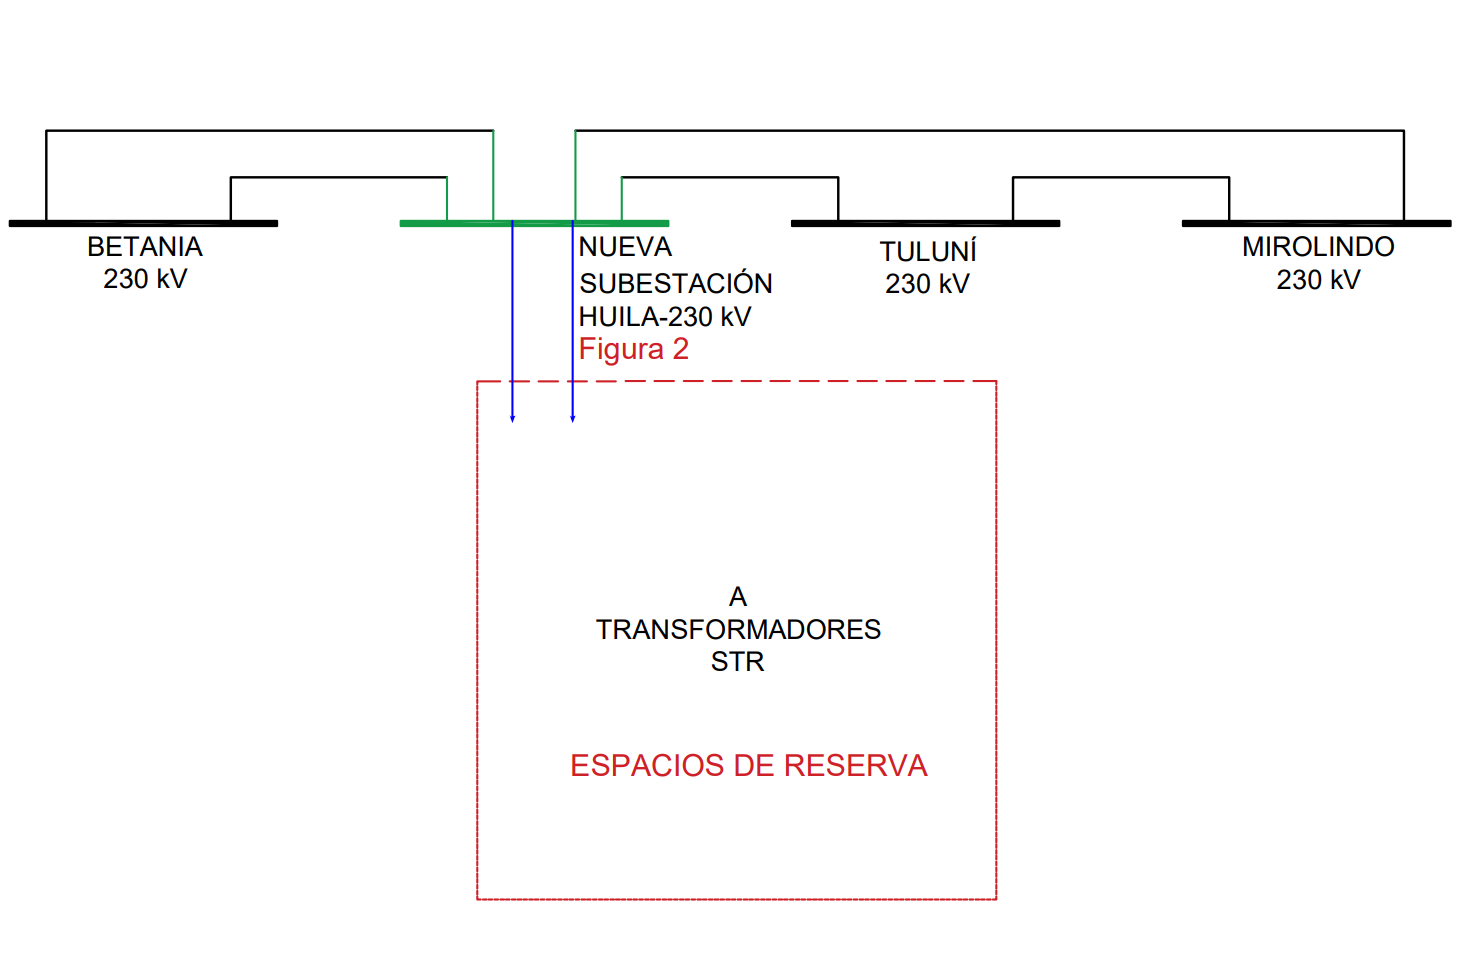
\includegraphics[width=1\textwidth]{1mer avance foticos/Esquema unifilar diagrama esquemático.png}
        \caption{en la figura del diagrama unifilar esquemático se logra evidenciar de una manera mas sencilla como ira conectada la nueva subestación Huila.} % Título de la figura
        \label{fig:Esquema} % Etiqueta para referencias
    \end{subfigure}
    \hfill % Espacio horizontal entre las subfiguras
    \begin{subfigure}{0.5\textwidth}
        \centering % Centra la imagen
        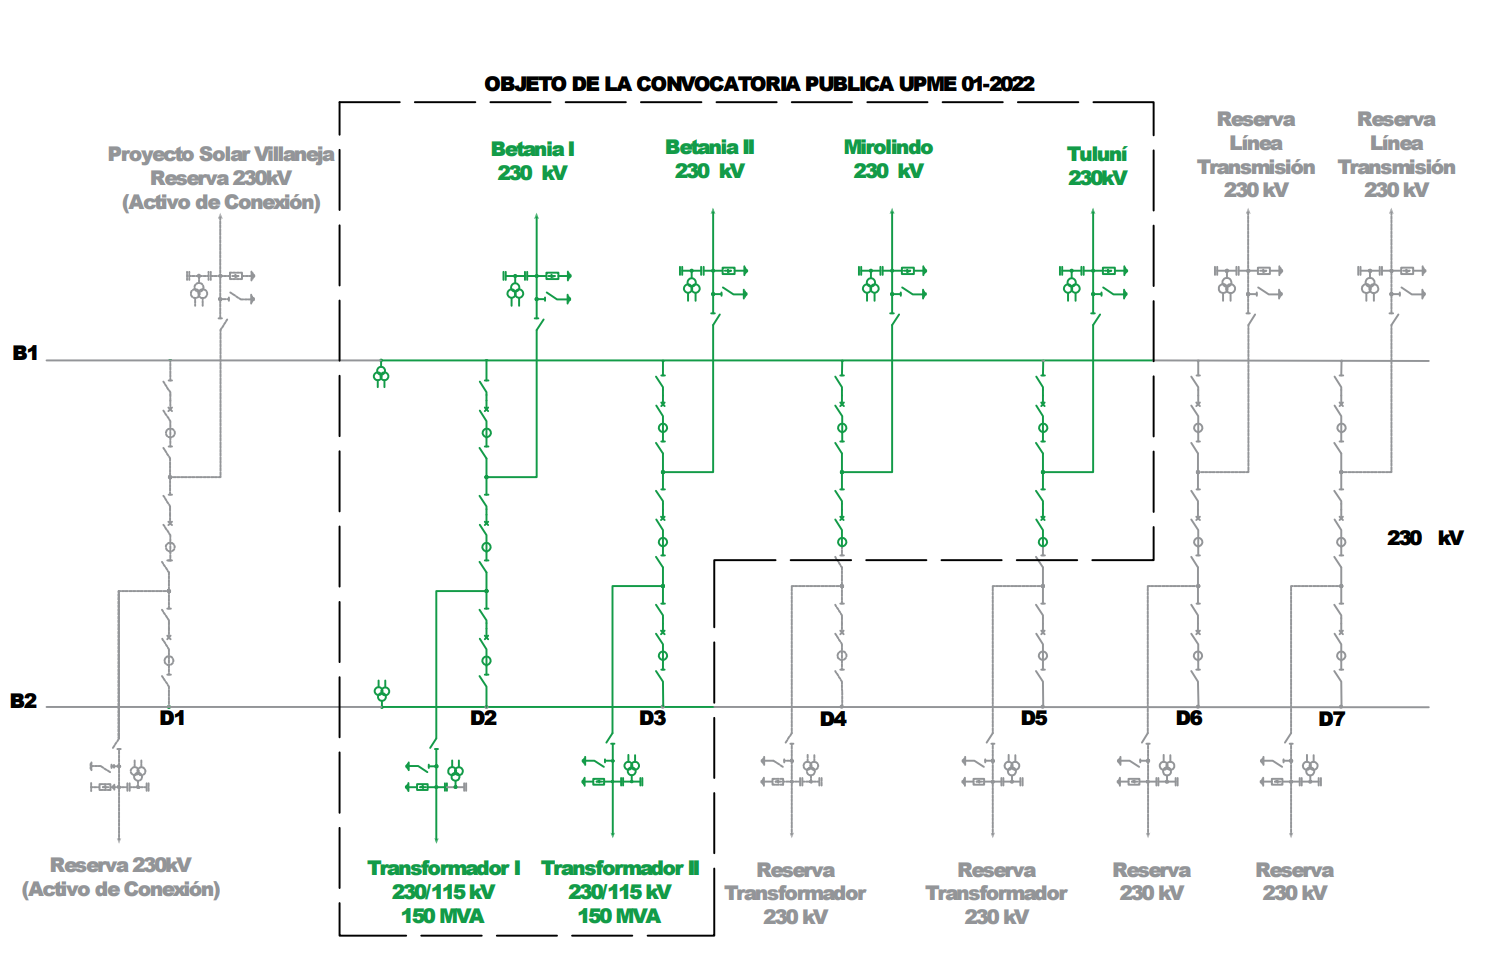
\includegraphics[width=1\textwidth]{1mer avance foticos/Esquema unifilar de la subestación huila 230kv.png}
        \caption{Esquema unifilar de la subestación huila 230kv.} % Título de la figura
        \label{fig:unifilar} % Etiqueta para referencias
    \end{subfigure}
    \label{fig:dos-imagenes}
\end{figure}

